
\subsection{Comparing Canada to the US}

\begin{figure}
    \centering 
    \caption{Inflow of Chinese immigrants to Canada and the US, as measured by the Canadian and US Censuses.}
    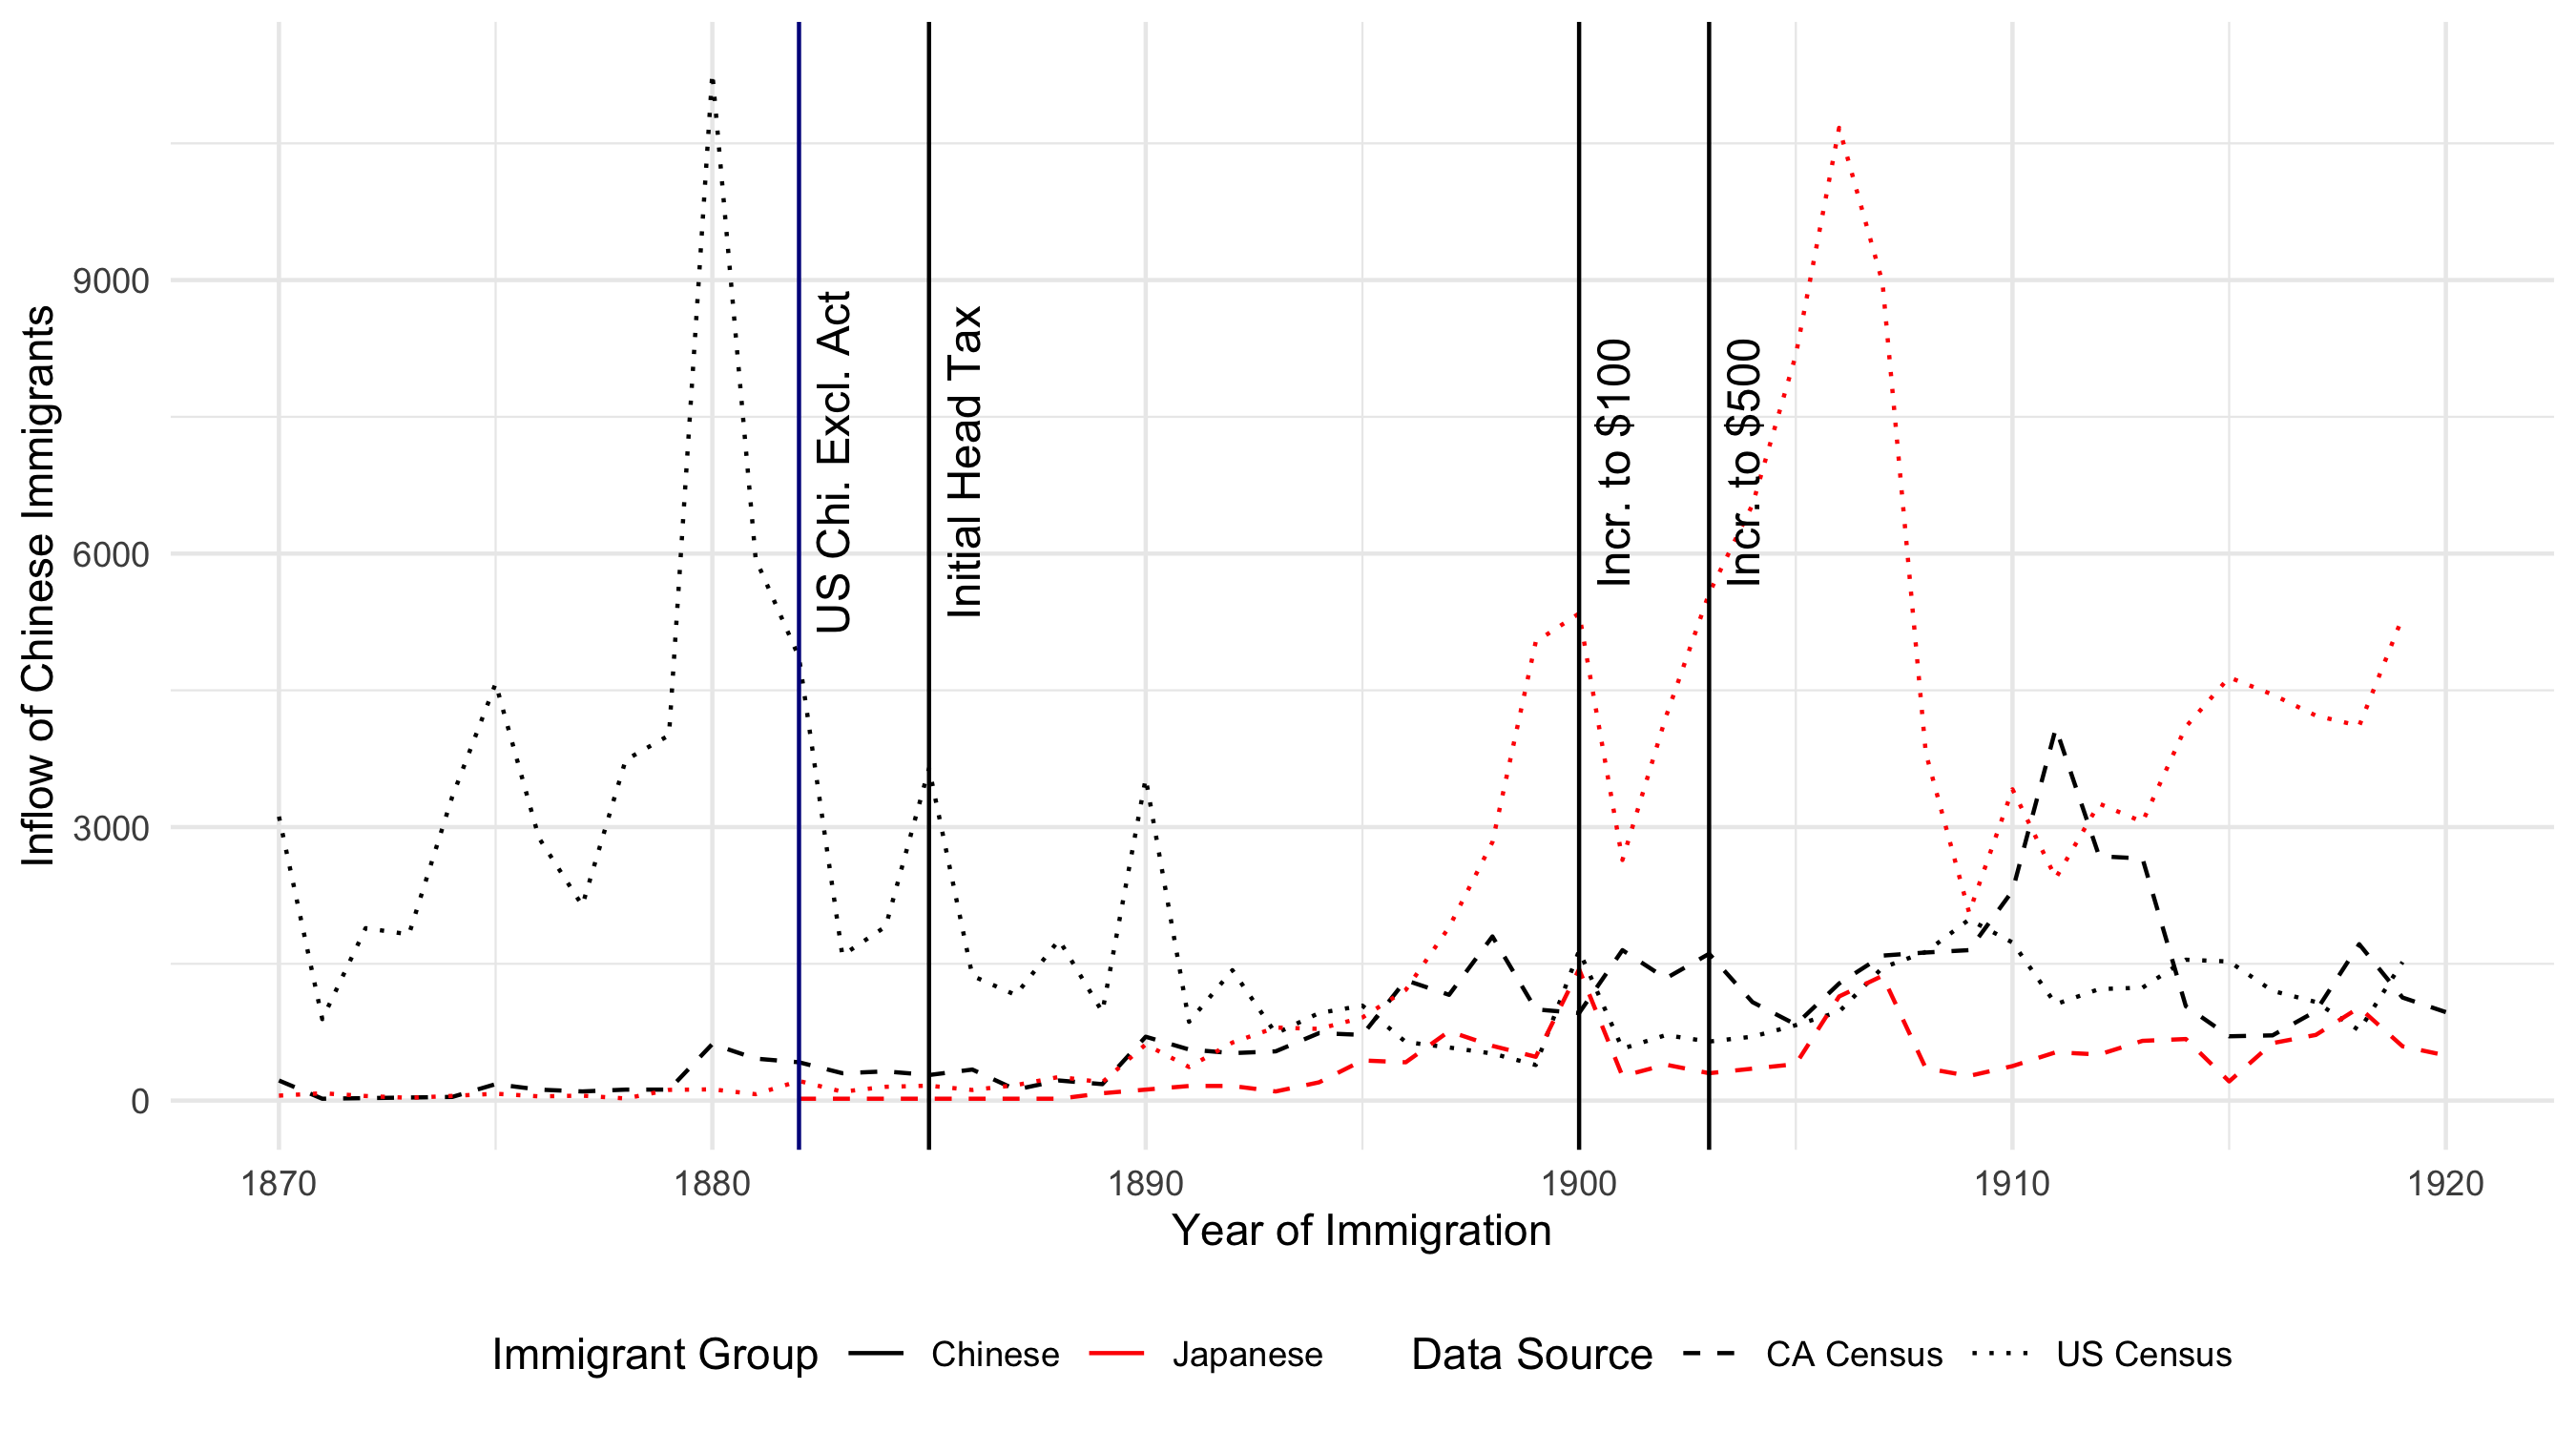
\includegraphics[width=\textwidth]{../../figs/fig3_us_can.png}
    \label{fig:taxpaid}
\end{figure}

The above analysis relies on the assumption above that in the absence of the head tax, the outcomes of Japanese and Chinese immigrants to Canada would have evolved similarly. In reality, it is likely that there were China-specific immigration shifters that would have affected Chinese immigration to Canada differently over time. In this section, I control for supply-side shocks by estimating the following equation:

\begin{multline}
    \label{eq:uscan}
    y_{ict} = \delta_{ct} + \sum_{c \in \{US, \, Canada\}} \alpha_c BORNCHI_i \times \mathbf{1}[COUNTRY_i = c] \\ + \sum_{k \in \{100,500\}, \, c \in \{US, \, Canada\}} \gamma_{ck} BORNCHI_i \times \mathbf{1}[COUNTRY_i = c] \times \mathbf{1}[TAX_t = k] + \varepsilon_{ict}
\end{multline}

where $c \in \{US, \, Canada\}$ indexes country, the coefficients $\alpha_c$ and $\gamma_{ck}$ now vary by country of arrival, and $\delta_{ct}$ now represents Year $\times$ Country fixed effects. 

\begin{table}[!h]
    \centering 
    \renewcommand{\arraystretch}{1.1}
    \resizebox{0.7\textwidth}{!}{
    \begin{threeparttable}
        \caption{Regression results from Equation \ref{eq:uscan} showing the relationship between the Chinese Head Tax and Chinese immigrant outcomes in Canada as compared to the US.}
        \label{tab:uscanregs}
        
% Table created by stargazer v.5.2.3 by Marek Hlavac, Social Policy Institute. E-mail: marek.hlavac at gmail.com
% Date and time: Sat, Apr 01, 2023 - 00:36:30
\begin{tabular}{@{\extracolsep{5pt}}lccc} 
\\[-1.8ex]\hline 
\hline \\[-1.8ex] 
 & \multicolumn{3}{c}{Sample: Chinese and Japanese Immigrants} \\ 
\cline{2-4} 
\\[-1.8ex] & LABORER & LITERATE & HOMEOWN \\ 
\\[-1.8ex] & (1) & (2) & (3)\\ 
\hline \\[-1.8ex] 
$BORNCHI \times US$ & $-$0.228$^{***}$ & $-$0.109$^{***}$ & $-$0.027$^{***}$ \\ 
& (0.009) & (0.007) & (0.006) \\ 
& & & \\ 
$BORNCHI \times CANADA $ & 0.252$^{***}$ & $-$0.057$^{***}$ & 0.041$^{***}$ \\ 
& (0.014) & (0.014) & (0.010) \\ 
& & & \\ 
$BORNCHI \times US \times $ \$100 Tax & 0.087$^{***}$ & 0.026$^{**}$ & $-$0.006 \\ 
& (0.014) & (0.012) & (0.010) \\ 
& & & \\ 
$BORNCHI \times US \times $ \$500 Tax & 0.062$^{***}$ & 0.048$^{***}$ & 0.012$^{*}$ \\ 
& (0.010) & (0.008) & (0.007) \\ 
& & & \\ 
$BORNCHI \times CANADA \times $ \$100 Tax & $-$0.256$^{***}$ & 0.298$^{***}$ & $-$0.114$^{***}$ \\ 
& (0.025) & (0.024) & (0.017) \\ 
& & & \\ 
$BORNCHI \times CANADA \times $ \$500 Tax & $-$0.112$^{***}$ & 0.010 & $-$0.118$^{***}$ \\ 
& (0.017) & (0.016) & (0.012) \\ 
& & & \\ 
Includes Year $\times$ Country FE & Yes & Yes & Yes \\ 
\hline \\[-1.8ex] 
Observations & 109,012 & 108,639 & 109,012 \\ 
Adjusted R$^{2}$ & 0.061 & 0.079 & 0.032 \\ 
\hline \\[-1.8ex] 
\end{tabular} 

        \begin{tablenotes}
            \item $^{*}$p$<$0.1; $^{**}$p$<$0.05; $^{***}$p$<$0.01
            \item 
            \item \textbf{Notes:} Analysis in this table uses Canadian census data from 1901-1921 and US census data from 1900-1920. As in Table \ref{tab:outcomes} I restrict the sample such that only immigrants who arrived after 1890 and prior to 1920 are included (since the latest US census year I use is 1920). All columns restrict the sample to only Chinese and Japanese immigrants from the US and Canada.
        \end{tablenotes}
    \end{threeparttable}
    }
\end{table}

Results of estimating Equation \ref{eq:uscan} for the sample of Chinese and Japanese immigrants to Canada who arrived between 1890 and 1920 are presented in Table \ref{tab:uscanregs}. Observe that Canadian Chinese immigrants are significantly less literate and more likely to be laborers than US Chinese immigrants, as suggested by summary statistics in Table \ref{tab:summstats}, and are also less likely to own their own home. Lines 3 and 4 represent the impact of Chinese immigrants to the US arriving in years with a higher \textbf{Canadian} head tax, which I would expect to be minimal, but I in fact observe to be significant. This suggests that the head tax may have had some spillover effects on Chinese immigration to the US. 

Column (1) shows that while Chinese immigrants to Canada in higher head tax years are less likely to be laborers (in line with the selection effect observed above), Chinese immigrants to the US in higher head tax years are in fact \textbf{more} likely to be laborers. This actually lends support to the selection theory, since the lower-skilled immigrants who could not afford the higher head tax may have substituted towards immigration to the US (although the existence of the Chinese Exclusion Act during this time period, which prohibited immigration of laborers, complicates this theory). 

Column (2) shows that immigrating in years with higher head taxes is associated with higher literacy rates for Chinese immigrants to both the US and Canada -- this is a puzzling result, as it does not accord with a theory of substitution between the US and Canada. Earnings are not included as an outcome variable because they are not available in the US census data during this time period, however column (3) presents results for home ownership. The results are again in line with my findings in Table \ref{tab:outcomes}, and the very small and mostly insignificant effects for Chinese immigrants to the US further suggests that the wealth effect (which does not affect Chinese immigrant outcomes in the US) dominates the selection effect (which would potentially spillover to Chinese immigrant outcomes in the US) for the outcome of home ownership.